\documentclass[12pt,openright,twoside,a4paper,english]{abntex2}
\selectlanguage{english}
\usepackage[utf8]{inputenc}
\usepackage{graphicx}
\usepackage{capa-epusp-abntex2/capa-epusp-abntex2}  % ver https://github.com/brunocfp/capa-epusp-abntex2/blob/master/README.md
% Folha de estilo: http://www.poli.usp.br/bibliotecas/servicos/publicacoes-online.html
% http://pro.poli.usp.br/wp-content/uploads/2012/04/NGTF2017.pdf
% http://www.poli.usp.br/images/stories/media/download/bibliotecas/DiretrizesTesesDissertacoes.pdf
% http://sites.poli.usp.br/d/pme2599/Documentos/Diretrizes%20de%20elabora%C3%A7%C3%A3o%20do%20trabalho%20final.pdf
\usepackage[alf]{abntex2cite}	% Citações padrão ABNT
\graphicspath{{./images/}}

\author{TIAGO KOJI CASTRO SHIBATA\\
HENRIQUE CASSIANO SOUZA BARROS\\
VICTORIA AKINA TANAKA}
\orientador{BRUNO DE CARVALHO ALBERTINI}
\areaconcentracao{Computer Engineering}
\preambulo{Monograph of the capstone project of the Computer Engineering bachelor in Escola Politécnica da Universidade de São Paulo}
\title{ColorMotion: Automatic video colorization}
\date{São Paulo\\(November 2018)}

\begin{document}
\begin{otherlanguage}{english}

\imprimircapa
\imprimirfalsafolhaderosto
\imprimirfolhaderosto

\begin{epigrafe}
\begin{flushright}
\vspace*{\fill}

\textit{``It is the supreme art of the teacher to awaken joy in creative expression and knowledge``}\\
(Albert Einstein)
\par\end{flushright}\end{epigrafe}

\begin{resumo}
Given a grayscale video, this paper proposes a method for colorization using convolutional neural networks in an encoder-decoder architecture. Unlike current image colorization models which, when applied frame by frame, create inconsistencies between frames, this model maintains some state between frames and learns to colorize while maintaining the colors of regions that existed on previous frames. The algorithm uses dense optical flow to propagate colors between frames. The method is user-guided in the sense that an user can input pixel colors as additional information, biasing the algorithm at multimodal color choices. Training was done on large scale datasets taken from open source videos and the ImageNet dataset, which was artificially augmented to generate frame sequences with motion.
\vspace{\onelineskip}

\noindent
\textbf{Keywords}: CNN. Colorization. Video. Restoration. Encoder-decoder.
\end{resumo}

TODO listas de gráficos, tabelas, abreviaturas e siglas, símbolos
\cleardoublepage

\tableofcontents

\maketitle

\chapter{Introduction}
In this paper, we propose a method for automatic video colorization, using a machine learning-based approach.

Previous work (TODO reference Colorful...) has used CNNs trained on large-scale datasets to colorize pictures successfully. However, when applied frame by frame on videos, the predictions have inconsistencies between frames, since no state is maintained between frames and different colors are predicted on the same object after small changes in the input grayscale image.

Since the colorization problem is multimodal (TODO reference Colorful), that is, multiple colors are plausible colorizations for a single object, the proposed model can also be user-guided. The algorithm can take input colors for a given object (e.g. the user can choose a t-shirt's color to be red) and will colorize the object and propagate it to the next frames.

\section{Motivation} \label{sec:Motivation}
The problem of colorization in the field of machine learning is one of major interest. It is not a solved problem and poses challenges unlike others, since its solutions are multimodal (the same object has multiple plausible colorizations) and its goal can be not to generate the colorization closest to ground truth, but one that's the most believable. Furthermore, it automates a manual, boring and expensive process: professional picture and video restoration services can cost upwards of thousands of dollars (TODO adicionar quote de empresas contatadas).

We take colorization of videos to be an extension of the colorization of images. We propose the use of state-of-the-art machine learning algorithms to colorize videos, prioritizing methods to maintain consistency of colors between frames in a scene whilst correctly colorizing new objects in a frame and detecting frames associated with a new scene. Our base model architecture is heavily based on previous image colorization work, with added state and an intermediate dense optical flow step. The intermediate dense optical flow step using the Lucas-Kanade method makes the model non-differentiable and, thus, not an end to end trainable CNN; however, we achieve good results training the encoder and decoder separately.

\section{Evaluation}
Results are trained on large scale data using open source videos, personal videos collected by the authors, and ImageNet images augmented to have artificial motion. (TODO insert loss imformation). The results are then tested on people: Volunteers were asked to rate scenes as original or computer colorized, so we can have a metric on how believeable the colorization is.

\section{Justification}
As stated in section \ref{sec:Motivation}, the traditional process of coloring images involve manual inputs from the user and use of advanced professional editing tools.
%TODO: citation needed, probably something about restoring pictures
The same can be said to the colorization of videos, with the added difficulty of maintaining consistency through frames. Some tools can help tracking the motion and colors between frames, but the initial input and challenges involving rapidly changing scenes add to the complexity of the process. (TODO: citar ferramentas atuais na industria)

\chapter{Related work}

TODO: Importar nossos resumos do Mendeley

1) Levantamento bibliográfico em bases de dados nacionais e internacionais, a
partir de palavras-chave em português e inglês;

2) Busca pelos textos completos dos trabalhos selecionados no levantamento;

3) Leitura e fichamento (resumo analítico) dos trabalhos relevantes. É imprescindível anotar os dados dos documentos consultados, para posterior citação e referência;

4) Cruzamento de informações e citações de modo a elencar um quadro de autores sobre o assunto, alinhados com o ponto de vista do pesquisador;

5) Redação da revisão e citações, de acordo com o assunto e tópicos abordados.

A learning-based approach for automatic image and video colorization

\chapter{Methodology}
\section{Conceptual aspects} \label{sec:Concept}
Neural networks for colorization can be divided in two broad categories: those that require a input from the user, and those that use a automated process. In both cases, the most common approach uses Convolutional Neural Networks (CNN) to leverage different image characteristics, and use those patterns to identify and separate objects in the image and colorize them accordingly. Other approaches are possible, for example through the use of self organizing maps along side neural networks as shown in Richart \textit{et al.} \cite{Richart_som_nn}; but for the purposes of this paper we will focus in CNN-based algorithms.

User guided algorithms TODO

\section{Methodology}
The methodology adopted four main phases of development: study and choice of existent machine learning algorithms; development of a dataset; adaptation of the chosen algorithm to support recurrent frame inputs and optical flow patterns; and optimization based on A/B tests and metrics.

% \subsection{Choice of algorithm}
% Like stated on section \ref{sec:Concept}, the

\section{Dataset}
\subsection{Colorspace}
As stated on Colorful (TODO: cite) and seen on related works, the L*a*b colorspace is most suitable for the colorization task. It's L* channel is the achromatic lightness quantity, which depends solely on the perceptually achromatic luminance. Thus, the perceptual lightness of a colorized image to a human observer appears most similar in lightness to a grayscale image when using the L*a*b* colorspace and maintaining the L* value. We use all network input images as a single channel L* image, and all color outputs are given in the a*b* colorspace.

\begin{figure}[!htb]
\centering
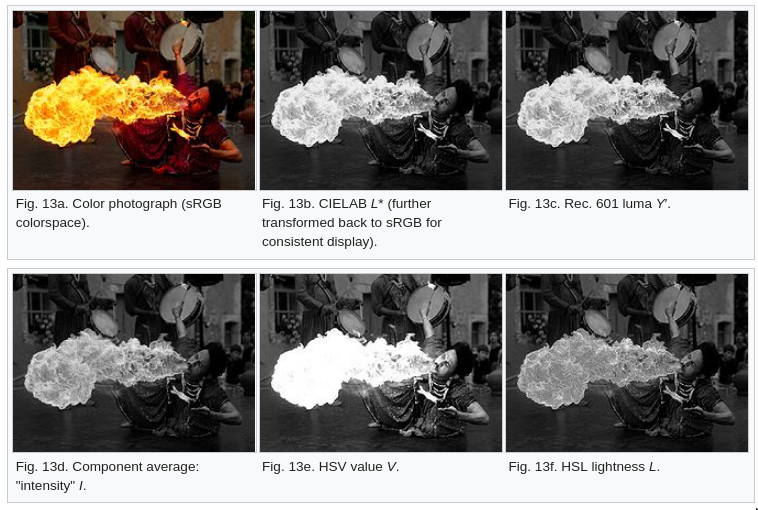
\includegraphics[width=\textwidth]{Colorspaces}
\caption{Source: https://en.wikipedia.org/wiki/HSL\_and\_HSV (TODO: adicionar como citação)}
\label{Label}
\end{figure}

\subsection{Processing of scenes from movies}
TODO adicionar citações dos filmes e links para páginas dos projetos

The initial dataset was composed of the open source movies Tears of Steel and Valkaama. After filtering and splitting the scenes, the dataset had 142753 frames in 836 distinct scenes.

To split the movies into independent scenes, two strategies were employed. We created a program to compute the structural similarity index (SSIM) between each pair of frames and, whenever the SSIM was high, we assumed a new scene was starting. The SSIM is similar to the simpler, less robust mean squared error (MSE) metric, but more resistant to noise and compression artifacts.

We also ran a histogram analysis on the pixel values of each frame and discarded frames without enough variability. This strategy removed introduction frames, black frames from fading effects, final credits and other undesired frames.

After running a script with both algorithms, the result was almost perfect. A few scenes that were cut into multiple scenes because of too fast movement (yielding a high SSIM in the same scene) were fixed after manual inspection.

TODO inserir curvas de perda dos testes iniciais em teste/validação

After initial training, this dataset proved too small for the task in hand. In our methodology, we employed a network with a high number of parameters, which is very prone to overfitting. The network did overfit a lot in our initial tests, as can be seen by the loss MSE of 4.21 and validation MSE of 98.43.

Augmentation:

TODO document Keras augmentation

The dataset was enlarged with videos from the free video repository Pixabay, under the Creative Commons licence, and from videos in the author's personal archives. The enlarged dataset has 591780 frames in 1629 distinct scenes. Data augmentation was also implemented during training to reduce the amount of overfitting to the training dataset. Augmentation was

TODO document augmentation. TODO show reduced overfitting, show loss curves.

Lastly, part of the ImageNet (ref: http://image-net.org/about-overview) dataset was downloaded from the URLs provided in the ImageNet website. The dataset has a variety of pictures belonging to one of thousands of "synonym sets". 895881 (TODO: update number) images were used during training of the user guided colorization model.

\subsection{Algorithm adaptation}
TODO: descrever arquitetura

TODO: descrever interpolação de features encodadas p/ manter estado do frame

TODO: descrever função de perda

TODO strategy: incremental enhancements and retraining, document importing weights from other models, document performance optimizations

\subsection{Optimization}
After these initial results, we achieved a validation MSE loss of 38.43 (TODO: atualizar quando resultado melhorar). Our initial training strategy was to start with a deep, large model and use model pruning techniques to remove layers that don't affect the result and compress the model while achieving similar performance. To this end, (TODO: documentar métodos usados de poda).

\section{Used technologies}
Keras, OpenCV, numpy

\section{System specifications}
TODO specs, performance analisys
Using a GTX1080 consumer level card, streaming the frames one by one (without batching) leads to inference times of 32ms in the unoptimized, large, deep model. Batching multiple frames yields average performance of up to 28ms/frame.

\chapter{Results}


\chapter{Discussion of achieved results}

\chapter{Conclusions}

\chapter{TODO glossary, appendix}

\bibliography{referencias.bib}
%\printbibliography

\end{otherlanguage}
\end{document}
